\makeatletter
%\newcommand{\rmnum}[1]{\romannumeral #1 }
%\newcommand{\Rmnum}[1]{\expandafter\@slowromancap\romannumeral #1@}
\makeatother
\ifpdf
\graphicspath{{Background/BackgroundFigs/PNG/}{Background/BackgroundFigs/PDF/}{Background/BackgroundFigs/}}
\else
\graphicspath{{Background/BackgroundFigs/EPS/}{Background/BackgroundFigs/}}
\fi

\chapter{Background}
	\label{chapter_background}
	
	Memory consistency and coherence are closely tied, since consistency establishes rules for coherence. Thus, coherence is largely a software/hardware implementation of consistency. Multiprocessor systems benefit from coherent shared memory, as data sharing between processing elements (PEs) is simpler. Conceptually, the simplest possible coherent system would be one where all PEs share one common memory. While perfectly plausible, this system would be highly inefficient due to contention and latency. These limitations are typically diminished by data caching.
	
	Cache memory accesses usually require multiple cycles, and off-chip requests are often in the hundreds of cycles \cite{Hennessy06}. Memory technologies are continuously improved, but the performance gap is still quite large. A hierarchical memory structure bridges the performance gap by masking memory latency. Caches are typically situated on the same substrate as the PEs. Lower memory latencies are achieved through physical proximity and smaller size. A multiprocessor system will typically have private caches for each PE, and a larger shared cache. Current architectures continue relying on this memory model. 
	
	Software parallelism is one way of improving overall performance, it has been the tendency over the past decade. Parallel software usually requires some communication between the distributed data and memory consistency dictates this communication behaviour. Typical coherence algorithms require explicit messaging between PEs. Most coherence schemes are highly sophisticated and require dedicated hardware resources.

	I have considered several memory coherence models when extending BERI to a multiprocessor design.
	Purely software or hardware coherence schemes are rarely implemented, so it is usually a tradeoff between the two mechanisms. Dedicated OS support is necessary for software coherence schemes and hardware assisted coherence is typically implemented through snooping or directory-based models. 
	
	In this chapter, I will first examine some software-based coherence schemes, followed by the motivations behind BERI directory-based coherence, and finally discuss coherence based on timestamps.

%\clearpage
	\section{Software Directed Coherence}
		User applications, particularly cross-platform applications, are usually designed to be oblivious to the memory architecture of underlying hardware. The same cannot be said for the operating system, which requires some knowledge of the cache layout, but subtle variations in cache design can still be concealed. The OS requires this information for general correctness and security. Instruction Set Architectures (ISAs) often supply the OS with special MMU instructions for cache control. MIPS provides a range of cache invalidation instructions.
		
		The OS may choose to explicitly invalidate cache lines, particularly when adding or removing kernel page tables \cite{Miller15}. This form of cache flushing is necessary due to possible aliasing arising from virtually indexed but physically tagged caches. Introducing new virtual-address-space mappings may lead to issues with larger caches. This form of OS driven memory consistency maintains a coarse grained memory state, however, parallel user applications often require fine grained support. Additionally, some instructions are restricted to kernel space, such as MIPS cache invalidate instructions.
		
		The general growth in compiler development and a better understanding of parallel software behaviour has made compiler-driven coherence both feasible and necessary. Modern systems often require software hints in order to achieve efficient and effective coherence, whether using strong or weak consistency models. 
		Various compiler-assisted memory coherence schemes have been proposed and evaluated, however, most designs still require some form of hardware support \cite{Lee98,Hwang96,Cheong88,Hoichi90,Choi94,Choi96,Choi00_0,Choi00_1,Fensch08}. 
		
		Hardware assisted software coherence designs mostly rely on cache self-invalidation, discussed in Section \ref{background_timebased}. 
		Software schemes evict stale data by inserting explicit cache invalidate instructions, evaluated using compile-time information. These techniques do not necessarily rely on specific OS support, but may employ similar coherence tracking routines. Several challenges arise from such coherence techniques:
		
		\begin{itemize}
			\item The compiler must carefully consider all operations; missing a cache invalidate will result in a possible deadlock, but aggressive invalidation will degrade performance.
			\item Some hardware assistance is still necessary; instructions for cache manipulation, message passing mechanisms, or time-based self-invalidation.
			\item Software cross-compilation and variations in hardware architecture could have a huge impact. For instance, a change in cache hit policy will significantly impact a software coherence model.
		\end{itemize}
		
		The behaviour of a cache write hit policy has a significant impact on the coherence design \cite{Smith82,Jouppi91_1,Chen92}. Write-through schemes are simpler to operate as invalidation of a local copy does not directly affect the lower cache levels; one disadvantage is an increase in memory traffic. Write-back schemes reduce overall memory traffic, but also introduce new coherency states. In contrast to write-back schemes, cache instructions may be necessary to ensure the propagation of updates into shared memory.
		
		Compiler-assisted coherence schemes have limitations, but in some cases they may be the only available option.
		The 80-Tile experimental processor was developed by Intel \cite{Vangal08,Mattson08}, used for evaluating processor scaling. The design did not have any hardware coherence support and required hand crafted software to demonstrate parallel behaviour. 
		The 80-Tile processor highlighted the challenges of designing hardware coherence, and the software complexity of a design without this support. 
		Future revisions of the design resulted in the 48-core SCC processor \cite{Mattson10}, with a return to more traditional hardware coherence support.
	
		Software directed coherence is challenging and requires a greater investment from the designer, a constant tradeoff between hardware and software developers. Commercial processors tend to provide some level of hardware coherence, and in many cases very strong support. 

%\clearpage
	\section{Directory-Based Coherence}
		Hardware coherence schemes are more common than purely software-based schemes, primarily due to some of the challenges and overheads associated with parallel software. Shared bus snooping schemes have been very popular in commercial multiprocessor designs, showing good performance and reasonable scaling for a small number of cores. 
		However, research has repeatedly shown that snooping does not scale beyond a small number of cores \cite{Hennessy06}. Directory-based coherence schemes have shown better scaling, supporting hundreds or thousands of cores using clever optimisations \cite{Martin12,Sanchez12}. 
		
		Shared resources rarely scale well and distributed memory designs such as chip multiprocessors (CMPs) are preferable \cite{Mullins04,Dally01}. Directory coherence can be applied to both shared memory designs and CMPs. Larger designs opt for distributed directories and allow for lower directory storage overheads. Typical producer-consumer sharing properties can constrain the number of tracked sharers and reduce global coherence communication \cite{Byrd99}.
		
		In recent years multiprocessor designs have become ubiquitous, offerings from Intel include larger designs with 15 cores in the Xeon E7 range \cite{xeon11} and $\sim$60 cores in the Xeon Phi range \cite{Rahman13}. The designs largely rely on snooping through ring buses, which naturally order messages, and other interconnects such as QPI \cite{Ziakas10}. 
		However, they still suffer communication latencies, especially coherence related traffic. Designers are constantly working on improving communication rates, efficiency of message distribution, and reduction in coherence traffic. 
		
		Historically directory-based coherence designs were incorporated into experimental multiprocessors such as the Stanford DASH and HYDRA \cite{Lenoski92,Hammond00}, based on early research into scalable coherence protocols \cite{Chaiken90,Agarwal88,Stenstrom90,Lilja93}. 
		Advantages of directory-based coherence over snooping and extensive related research, were my motivations for selecting this protocol as the default BERI multiprocessor coherence model.
		
		The BERI directory protocol uses a full-map directory implementation such as the one described by Chaiken et al. \cite{Chaiken90}. Numerous other directory variants exist, which can provide a more efficient directory distribution. However, the simplicity of the dual-core system has allowed me to use this scheme, as bandwidth, and communication overheads are less visible.
		
		Latency is problematic for coherence designs enforcing strong or strict memory consistency and communication overheads can become a serious limitation. Cheng et al. \cite{Cheng94} have highlighted major drawbacks in directory protocols: tracking ownership of every cache line, explicit individual line invalidation requests, blocking on release operations, coherence actions due to line requests, and multi-level cache inclusion policy. Ros et al. \cite{Ros12} have demonstrates the need for coherence traffic reduction in large distributed systems.
	
%\clearpage
	\section{Time-Based Coherence}
		\label{background_timebased}

		The drawbacks of traditional message-based coherence protocols have lead me to explore alternative ways of maintaining coherence. 
		Specifically, a hardware coherence system following some standard memory consistency model and running unmodified commodity software. 
		I have already mentioned that memory consistency schemes strongly affect coherence models. The distinction between hardware and software coherence is blurred when using weaker models, so could a weak memory model eliminate coherence messaging altogether? 

\clearpage
		This question is definitively answered by the time-based cache coherence model. This scheme associates each cached memory line with a timestamp.
		The validity of cached data is evaluated through time fragmentation, where cache lines are valid for a fixed time period. Expired memory lines are updated using the normal cache fill mechanisms.
		
		Cache coherence based on time is not a new concept in itself, variations of this mechanism have been described in related work \cite{Keleher94,Shim11,Lis11,Yu15_0,Yu15_1,Kurian15,Singh13,Singh14,Elver14}.
		Most designs use the timestamp mechanism in conjunction with other coherence schemes such as snooping or directories.
		However, early research into timestamp-based coherence has suggested that a standalone system based on this scheme should be possible. Evaluation of these designs were limited to fairly basic simulation and hardware approaches, and heavily relied on the correct behaviour of the compiler. Additionally, the systems were evaluated using select code snippets that were easier to evaluate and analyse.
		
			\subsection{Early Research}
				Original designs of time-based coherence schemes were largely limited by minimal software support for relaxed memory. Stale data was the primary concern for program correctness, and explicit cache invalidation instructions were inserted by the compiler; demonstrated by Cheong and Veidenbaum \cite{Cheong88,Hoichi90}. These instructions branched into two major categories, TLB-based invalidates and compiler inserted. 
				
				The TLB approach was potentially wasteful as entire pages were deemed invalid. However, recent research on optimised TLB self-invalidation has been proven effective; demonstrated by Gutierrez et al. \cite{Gutierrez12}. This scheme is aimed at JIT compiled self-modifying code.
				
				The compiler approach is finer grained but overheads due to explicit cache flushing may be costly. The compiler identifies loads and stores to shared data at compile-time.
				The cached data is explicitly tagged with additional bits, indicating whether it is private or shared. Cache invalidate instructions are then used to clear the cache of stale data at the end of subroutines; each new subroutine is expected to start with a clean cache.
		
			\subsection{Compiler-Assisted Approach}
				Timestamp-based coherence (TS) was originally proposed by Min and Baer \cite{Min92} and later improved by Xin et al. \cite{Xin96}. This approach relies on compile-time software analysis and some additional hardware support. In this scheme, cache lines are tagged with additional time bits. The compiler analyses write operations and identifies shared data regions. 
				Each shareable data structure is associated with a clock, which is incremented at the end of the time epoch. If a cache line tagged with the previous epoch value is accessed, it is self-invalidated and a new copy is fetched.
				
				The clock counters used by the timestamp scheme can overflow. Some remaining stale data can still match a valid future epoch, thus, a full cache flush is necessary. This leads to a compromise between the number of bits used per cache line and the penalty of overflows. Darnell and Kennedy \cite{Darnell93} have shown that tag overheads can be reduced to 1 bit per line, however, the clock overflow constraints remain. 
				
				Authors do not mention the consistency policy of TS or its variants, but judging by their fear of stale data values, it is likely to be a strong consistency model. The BERI time-based protocol is somewhat similar to this description, however, unlike TS, the epochs are not compiler inserted, instead they are driven by the hardware and the compiler has no knowledge of them.
				
				%Cache invalidation comes in two flavours: indiscriminate and selective. Indiscriminate cache invalidation clears the entire cache, which can be done as a single cycle operation, at the cost of higher miss-rates for still useful data \cite{Darnell93}. Selective invalidation produces much lower miss-rates but requires sequential invalidation of cache lines which is expensive. My time-based model does both of these, as it selectively invalidates cache lines based on their individual time stamp expiry's, as well as a single cycle full cache flush on synchronisation instructions.

				\begin{figure}[t]
					\centering 
						\makebox{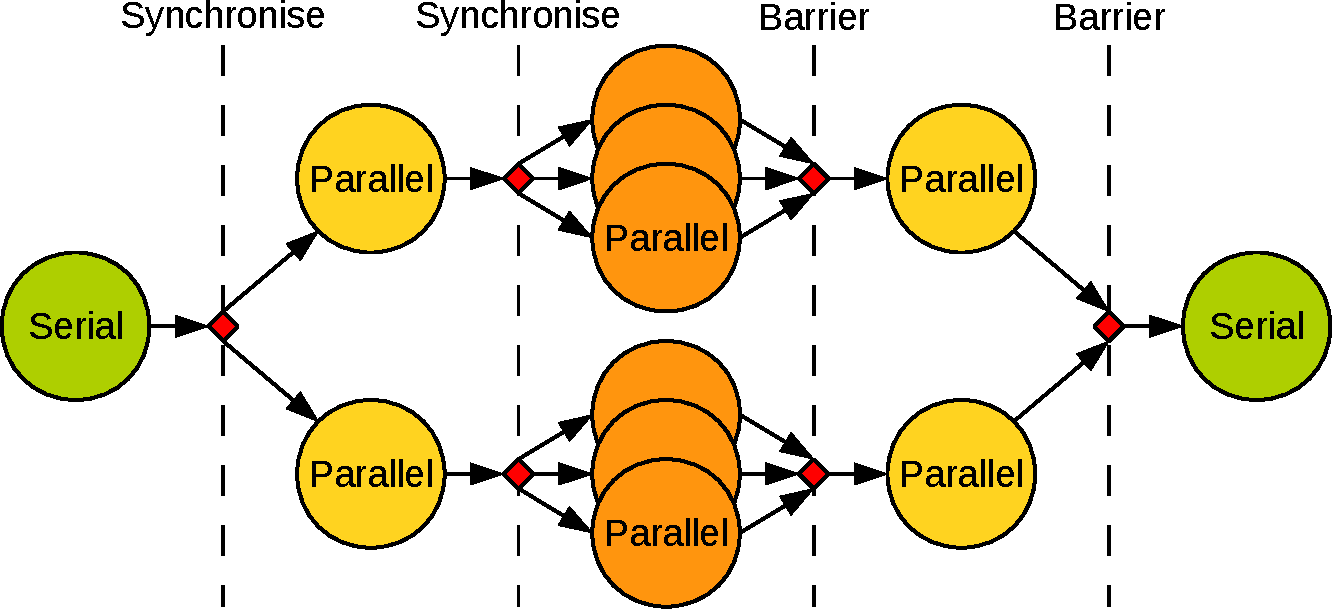
\includegraphics[width=\textwidth,height=\textheight,keepaspectratio]{software_sync}}
						\caption{Parallel software behaviour} 
						\label{software_sync}
				\end{figure}
				
				Figure \ref{software_sync} is a conceptual representation of generic parallel software behaviour \cite{Choi00_0,Choi00_1}. Most coherence schemes based on time, rely on this behaviour. The synchronisation and barrier points can be effectively exploited by the compiler or hardware to achieve global consistency; elaborated by Fensch \cite{Fensch08}.

				Hardware designs can be simplified through improved compiler support and better exploitation of data spacial and temporal locality. Such a design can provide coherence support to systems without hardware coherence, such as the Cray T3D processor, as demonstrated by Choi et al. \cite{Choi94,Choi96,Choi00_0,Choi00_1}. 
				Similar to TS, their coherence scheme associates timestamps with memory locations. However, their design relies on a special time-read instruction which checks memory location timestamps.
				This compiler inserted instruction, is aware of the most recent write to a memory location, and if the targeted memory location is older than the write, it is invalidated. 
				By the authors own description, this system mostly relies on correct compiler analysis. 
			
		
			\subsection{Hardware-Assisted Approach}
				There have been a number of proposals combining directory or snooping protocols with some form of timestamp coherence \cite{Lebeck95,Lai00,Yu15_0,Yu15_1,Kurian15}. These designs display an improvement over the base protocol and most of them enforce a strict memory consistency policy.

				In recent work by Elver and Nagarajan \cite{Elver14}, timestamps are added to memory locations as a means of reducing coherence communication overheads. Their scheme lowers the memory overheads of a MESI protocol by eliminating the sharing vector in shared memory, instead, the protocol tracks the current owner core. To compensate for an increase in coherence messages due to limited tracking, timestamps are added to the local and shared caches. 

				Further modification of directories using timestamps have been shown in \cite{Shim11,Choi11,Sung15}. Most of this work is based on MESI style directories for x86, and strong consistency models. 
				Another potential use for time-based coherence aimed at GPUs has been shown by Singh et al. \cite{Singh13,Singh14}. Traditionally, GPUs support little or no coherence. The authors have shown that self-invalidating GPU caches can improve overall performance. 

				A number of schemes based on Lamport \cite{Lamport78} vector clocks have also been explored. Keleher et al. \cite{Keleher94} have demonstrated vector clock style communication, lazy memory consistency, communicating over Ethernet. In order to achieve good performance their system is highly optimised to reduce memory coherence communication. A relaxed memory consistency design has allowed them to batch memory operations and reduce the impact of false sharing. 
				
				Lis and Shim \cite{Shim11,Lis11} have proposed the concept of Library Cache Coherence (LCC), which allows caches to check out data for a fixed amount of time. The scheme is based around a global clock which enforces sequential consistency (SC). Hardware support for strong memory consistency schemes such as SC is usually challenging and costly, however, an efficient implementation of this scheme is desirable. SC significantly reduces software complexity. 
				
				The LCC scheme removes the need for multicast or broadcast invalidations, typically required in directory-based schemes. LCC efficiency relies on an appropriate choice of data lending period, effectively a cache line time-out; a short lending period increases cache misses, and long time-outs cause delays as cores wait for lines to expire. 
				
			\subsection{BERI Time-Based Approach}
				The time-based scheme discussed in this dissertation avoids explicit cache coherence messages. 
				This scheme relies solely on cache self-invalidation, and correct use of software synchronisation and locking mechanisms. 
				The coherence model complies with a well defined relaxed memory consistency scheme (RMO{\large$^\star$}) \cite{SPARCInternational94}, thus, providing strong programmer assurances (discussed in Section \ref{section_rmo}).
				
				In contrast to other related designs discussed in this section, the BERI time-based coherence scheme is designed to function as a standalone system and does not require any changes to the operating system, compiler, or the ISA. I evaluate this model on a full system design in hardware, unlike the related work which is demonstrated predominantly using software simulations.
				
				Very few related designs have been verified against a memory consistency model, they mostly rely on the observed software interactions to determine the consistency behaviour. More crucially, I demonstrate that common operating systems and compilers already include the support for such a coherence and consistency design.

%\clearpage
\section{Memory Consistency}
	\label{background_consistency}
		
	A memory consistency model defines the behaviour of memory operations and provides programmer guarantees. A consistency model is generally more critical in multiprocessor systems where memory operations originate from different processing elements. Memory consistency is usually described through strictness of memory operations, strong consistency implies limited reordering of operations by the memory subsystem, a relaxed model offers more freedom in this respect. 
	
	Strong models are conceptually easier to understand, their behaviour is more predictable and may be sequential. Models such as Total Store Order (TSO) or Sequential Consistency (SC) require hardware support, but software support may be less complex. Relaxed consistency permits various non-chronological orderings of memory operations. Software design requires careful planning in order to support Relaxed Memory Order (RMO), while hardware support is reduced.

	Architectures such as x86 and its variants generally provide strong memory consistency such as TSO. As a result programmers are guaranteed that all store operations will commit in some fixed chronological order, and will be concurrently observable to the entire system. Maintaining this memory behaviour requires extensive hardware support, coordinating appropriate synchronisation messaging.
	
	Processor designs such ARM or PowerPC demonstrate a different approach to memory consistency design \cite{Sarkar11,Maranget12}. Both systems opt for a relaxed memory behaviour. Explicit synchronisation instructions are used to maintain a global memory order. Hardware complexity is reduced, since memory communication is not forced to follow a particular pattern. This memory behaviour relies on the fact that most software is written to run independently and merge at specific intervals; previously displayed in Figure \ref{software_sync}.

	
	\subsection{Memory Consistency Trace Format}
		\label{mem_format}
	
		I have used the AXE and CHERI Litmus model checkers developed by Matthew Naylor \cite{AXE_checker,CHERI_litmus} to evaluate the memory consistency behaviour of time-based and directory coherence. AXE is a trace checker, and BlueCheck \cite{bluecheck} is used to stimulate the memory subsystem with random inputs. The memory trace format used by the model checker is shown in Equation \ref{test_mem_trace_format}. It reports whether or not a given trace satisfies one of its supported memory models.
	
		\begin{equation}
			C_{id}: \ M[M_{addr}] \ \risingdotseq \ \mathbb{N}
		\label{test_mem_trace_format}	
		\end{equation}
		
		
		\begin{table}[!h]
		\begin{center}
		\begin{tabular}{|c|l|}
			\hline
			C$_{id}$: & Core/Thread ID \\
			\hline
			M[\ \ ] & Memory operation (SYNC is a variant) \\
			\hline
			M$_{addr}$ & Address of the memory operation \\
			\hline
			$\risingdotseq$ & Memory operation type \\
			& Load (==), Store (:=) \\
			\hline
			$\mathbb{N}$ & Natural number stored/loaded \\
			\hline
		\end{tabular}
		%\caption{}
		\label{test_mem_trace_format_legend}
		\end{center}
		\end{table}
	
	\subsection{Defining Memory Consistency}
		The memory consistency models evaluated by AXE are defined in this section.
		 %The model checking tool (AXE) analyses memory traces for a given memory architecture, the traces are evaluated and matched against a consistency model, described further.

		\subsubsection{Sequential Consistency} 
			This consistency model was defined by Lamport \cite{Lamport79}: ``The result of any execution is the same as if the operations of all processors were executed in some sequential order, and the operations of each individual processor appear in this sequence in the order specified by its program.''

		\subsubsection{Total Store Order}
			The Oracle{\tiny{$^{\textregistered}$}} information library \cite{Oracle15} defines this memory model as: ``TSO guarantees that the sequence in which store, flush, and atomic load-store instructions appear in memory for a given processor is identical to the sequence in which they were issued by the processor.''
			
			\captionsetup[table]{name=Trace}
			\begin{table}[!hb]
			\begin{center}
			\fontfamily{pcr}\selectfont
			\begin{tabular}{|l|l|}
				\hline
				\multicolumn{1}{|c|}{\textbf{TSO Trace}} & \multicolumn{1}{c|}{\textbf{MIPS Assembler}} \\
				Init (x==0, y==0) & Init addresses (x) and (y) \\
				\hline
				0: x := 1 & ``li r1, 1 ; sw r1, 0(x)'' \\
				\textbf{\textcolor{ForestGreen}{0: y == 0}} & lw r2, 0(y) \\
				1: y := 1 & ``li r1, 1 ; sw r1, 0(y)'' \\
				\textbf{\textcolor{ForestGreen}{1: x == 0}} & lw r2, 0(x) \\
				\hline
				\multicolumn{2}{|c|}{\textbf{\textcolor{ForestGreen}{Allowed}}} \\
				\hline
			\end{tabular}
			\caption[TSO consistency compliance]{TSO consistency compliance (\textit{Note: Instruction sequences for each core are listed in program order, however, the relative ordering between the two cores is variable})}
			\label{tso_compliance}
			\end{center} 
			\end{table}
			\captionsetup[table]{name=Table}
			
			\captionsetup[table]{name=Trace}
			\begin{table}[!hb]
			\begin{center}
			\fontfamily{pcr}\selectfont
			\begin{tabular}{|l|l|}
				\hline
				\multicolumn{1}{|c|}{\textbf{TSO Failure}} & \multicolumn{1}{c|}{\textbf{MIPS Assembler}} \\
				Init (x==0, y==0) & Init addresses (x) and (y) \\
				\hline
				0: x := 1 &  ``li r1, 1 ; sw r1, 0(x)'' \\
				0: sync & sync (barrier) \\
				\textbf{\textcolor{red}{0: y == 0}} & lw r2, 0(y) \\
				1: y := 1 & ``li r1, 1 ; sw r1, 0(y)'' \\
				1: sync & sync (barrier) \\
				\textbf{\textcolor{red}{1: x == 0}} & lw r2, 0(x) \\
				\hline
				\multicolumn{2}{|c|}{\textbf{\textcolor{red}{Disallowed}}} \\
				\hline
			\end{tabular}
			\caption{TSO consistency non-compliance}
			\label{tso_non_compliance}
			\end{center} 
			\end{table}
			\captionsetup[table]{name=Table}

			
			Trace \ref{tso_compliance} shows a memory ordering example satisfying TSO conditions. TSO permits the writes to \textbf{(x)} and \textbf{(y)} to be buffered locally at each hardware thread, allowing the subsequent loads of \textbf{(x)} and \textbf{(y)} to execute before the writes have reached shared memory. The loads to those addresses are permitted to observe initial values even after an update.

			Trace \ref{tso_non_compliance} shows TSO non-compliance. The synchronisation instructions force the writes to \textbf{(x)} and \textbf{(y)} to be flushed to shared memory before the subsequent loads of \textbf{(x)} and \textbf{(y)} can be performed. This example does not comply with any memory consistency model described in this dissertation.
			
		\subsubsection{Partial Store Order}
			The Oracle{\tiny{$^{\textregistered}$}} information library \cite{Oracle15} defines this memory model as: ``PSO does not guarantee that the sequence in which store, flush, and atomic load-store instructions appear in memory for a given processor is identical to the sequence in which they were issued by the processor. The processor can reorder the stores so that the sequence of stores to memory is not the same as the sequence of stores issued by the CPU.''
			
			Trace \ref{pso_compliance} shows a memory ordering scenario permitted by PSO. Both updates of \textbf{(x)} and \textbf{(y)} are performed by the same core, however, writes may be buffered and propagated in different orders. Thus, two load operations on another core may observe the memory values out-of-order.
			
			\captionsetup[table]{name=Trace}
			\begin{table}[!h]
			\begin{center}
			\fontfamily{pcr}\selectfont
			\begin{tabular}{|l|l|}
				\hline
				\multicolumn{1}{|c|}{\textbf{PSO Trace}} & \multicolumn{1}{c|}{\textbf{MIPS Assembler}} \\
				Init (x==0, y==0) & Init addresses (x) and (y) \\
				\hline
				0: x := 1 & ``li r1, 1 ; sw r1, 0(x)'' \\
				0: y := 1 & sw r1, 0(y) \\
				1: y == 1 & lw r1, 0(y) \\
				\textbf{\textcolor{ForestGreen}{1: x == 0}} & lw r2, 0(x) \\
				\hline
				\multicolumn{2}{|c|}{\textbf{\textcolor{ForestGreen}{Allowed}}} \\
				\hline
			\end{tabular}
			\caption{PSO consistency compliance}
			\label{pso_compliance}
			\end{center} 
			\end{table}
			\captionsetup[table]{name=Table}

		\subsubsection{Relaxed Memory Order}
			\label{section_rmo}
			This model further relaxes the rules on ordering of load and store operations; loads can be reordered with respect to other loads and stores to different addresses. Explicit synchronisation instructions are used to maintain a global order. Dependencies imposed by the memory subsystem can also affect the consistency model. 
			
			The SPARC--V9 architectural manual \cite{SPARCInternational94} states the following: ``Dependence order is a partial order that captures the constraints that hold between instructions that access the same processor register or memory location.'' Thus, two flavours of RMO exist, with and without dependencies. RMO with dependencies is a subset of RMO without dependencies. The PowerPC memory model falls somewhere in between the two, being stronger than RMO without dependencies but weaker than RMO with dependencies.

			\begin{figure}[t]
				\centering 
					\makebox{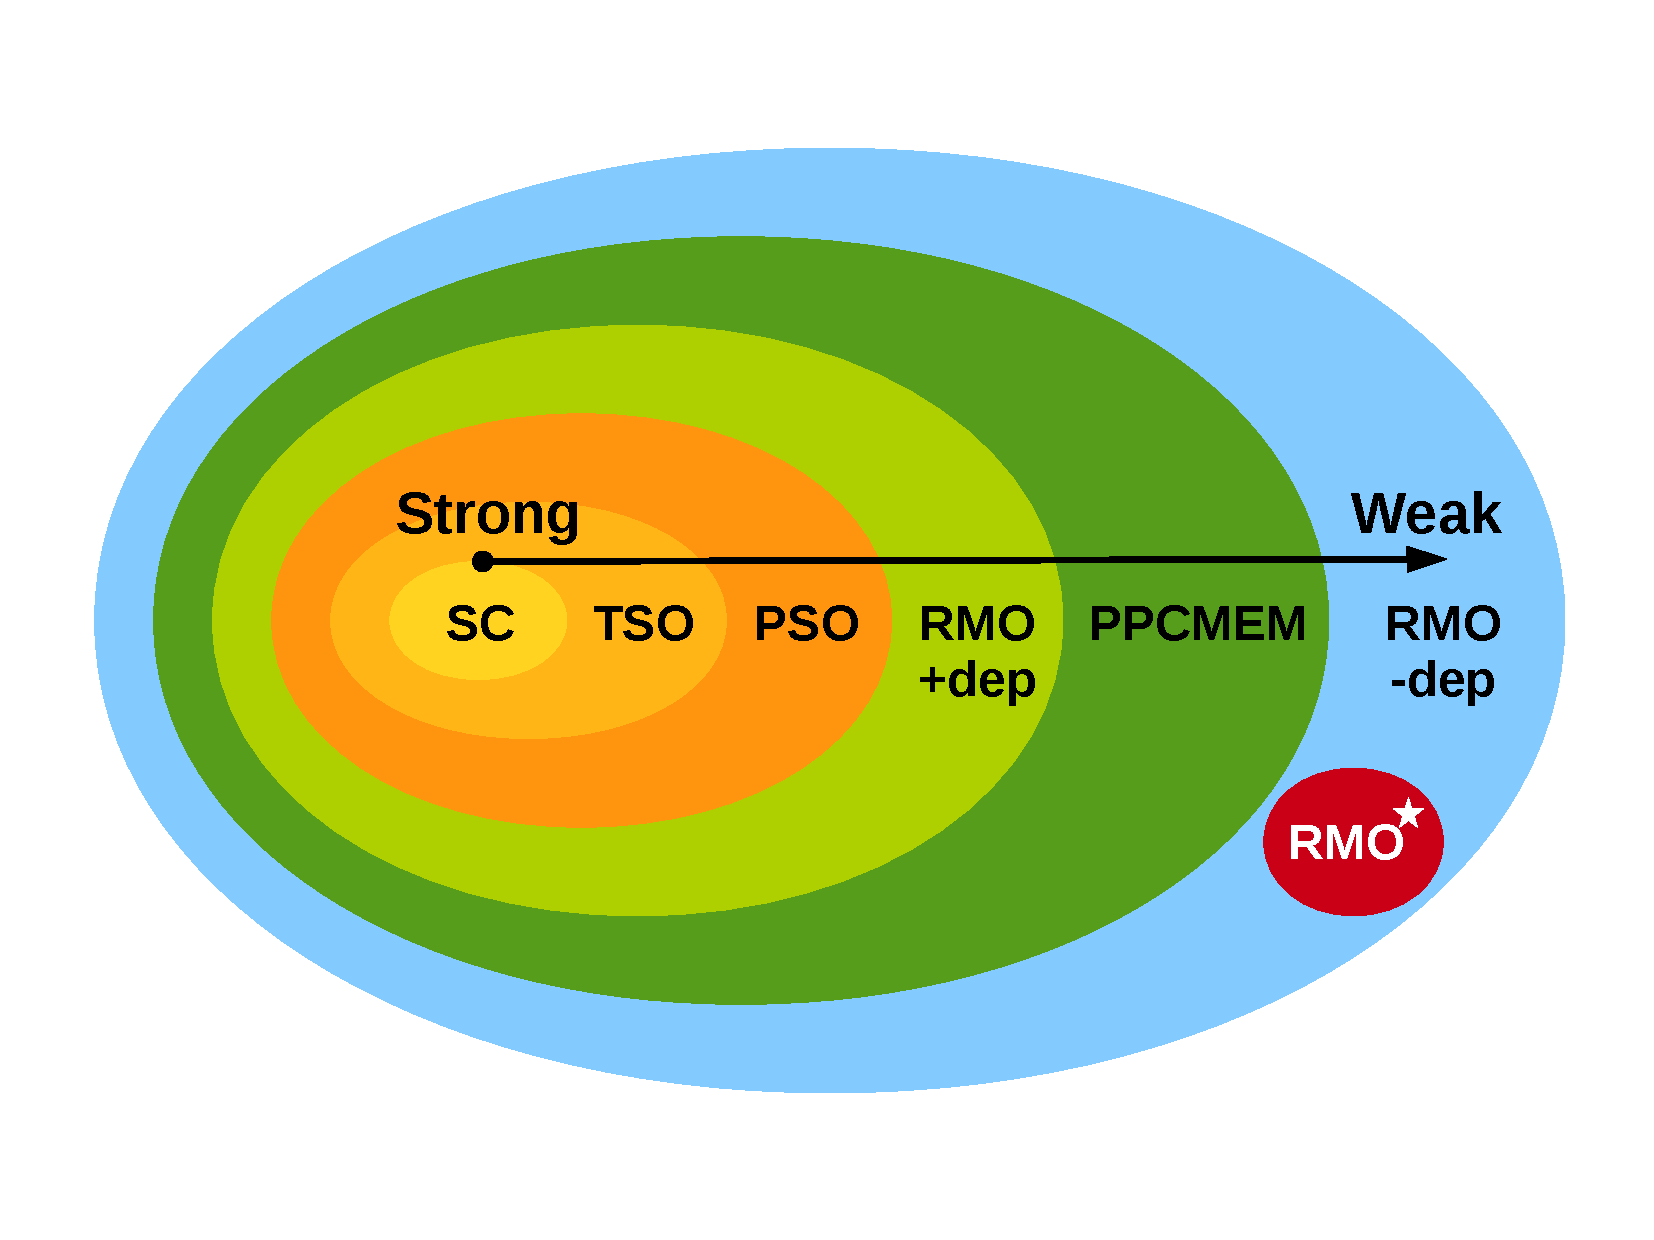
\includegraphics[trim={0 1.8cm 0 1.8cm},clip,width=0.75\textwidth,height=0.75\textheight,keepaspectratio]{consistency_sets}}
					\caption[Memory consistency model hierarchy]{Memory consistency model hierarchy. (\textit{Note: [+dep] and [--dep] indicate model evaluation with and without dependencies, respectively})} 
					\label{consistency_sets}
			\end{figure}
	
			\captionsetup[table]{name=Trace}
			\begin{table}[b]
			\begin{center}
			\fontfamily{pcr}\selectfont
			\begin{tabular}{|l|l|}
				\hline
				\multicolumn{1}{|c|}{\textbf{RMO Trace}} & \multicolumn{1}{c|}{\textbf{MIPS Assembler}} \\
				Init (x==0, y==0) & Init addresses (x) and (y) \\
				\hline
				0: x := 1 & ``li r1, 1 ; sw r1, 0(x)'' \\
				0: sync & sync (barrier) \\
				0: y := 1 & sw r1, 0(y) \\
				1: y == 1 & lw r1, 0(y) \\
				\textbf{\textcolor{ForestGreen}{1: x == 0}} & lw r2, 0(x) \\
				\hline
				\multicolumn{2}{|c|}{\textbf{\textcolor{ForestGreen}{Allowed}}} \\
				\hline
			\end{tabular}
			\caption{RMO consistency compliance}
			\label{rmo_compliance}
			\end{center} 
			\end{table}
			\captionsetup[table]{name=Table}
	
			The time-based coherence model described in this dissertation falls under RMO without dependencies, for convenience it will be referred to as \textbf{RMO{\large$^\star$}}. Figure \ref{consistency_sets} shows a hierarchy of memory consistency models based on strength, from strict to relaxed consistency. Examples of litmus tests shown in Chapter \ref{chapter_validation}, highlight the nuances in RMO{\large$^\star$} behaviour. 
			%The model has been checked with the complete AXE litmus test suite, as well as CHERI litmus tests. These tests have shown that RMO{\large$^\star$} falls under RMO without dependencies and does not violate any properties of this consistency model.
			
			Trace \ref{rmo_compliance} shows an example of RMO behaviour, the synchronisation instruction forces the writes to be performed in order, but now the loads can execute out-of-order, hence, this behaviour is allowed under RMO but not PSO. Core 1 does not perform any synchronisation operations, thus, both updated and stale values may be observed.
			
			\captionsetup[table]{name=Trace}
			\begin{table}[!h]
			\begin{center}
			\fontfamily{pcr}\selectfont
			\begin{tabular}{|l|l|}
				\hline
				\multicolumn{1}{|c|}{\textbf{RMO No Dependencies}} & \multicolumn{1}{c|}{\textbf{MIPS Assembler}} \\
				Init (x==0, y==0) & Init addresses (x) and (y) \\
				\hline
				0: x := 1 & ``li r1, 1 ; sw r1, 0(x)'' \\
				0: sync & sync (barrier) \\
				0: y := 1 & sw r1, 0(y) \\
				\textbf{\textcolor{BurntOrange}{1: y == 1 (block)}} & ``lw r1, 0(y) ; xor r3, r1, r1'' \\
				\textbf{\textcolor{ForestGreen}{1: x == 0}} & lw r2, \textbf{\textcolor{BurntOrange}{r3}}(x) \\
				\hline
				\multicolumn{2}{|c|}{\textbf{\textcolor{ForestGreen}{Allowed}}} \\
				\hline
			\end{tabular}
			\caption{RMO compliance, without dependencies}
			\label{rmo_no_dep_compliance}
			\end{center} 
			\end{table}
			\captionsetup[table]{name=Table}
			
			Trace \ref{rmo_no_dep_compliance} is an example of RMO compliance but only applicable when the memory subsystem does not block operations (without dependencies). If the system were to block the load of \textbf{(y)}, then only an updated value of \textbf{(x)} would be observed. This does not happen in RMO without dependencies (RMO{\large$^\star$}). 
			
			An advantage of a weak memory model is that it can be made stronger through synchronisation instructions, however, a strong model cannot be made weaker. It may be easier to design applications for strong models but the flexibility of weak models may be lost.

%\clearpage
\section{Cache Side-Channel Attacks}
	Contention for a hardware resource may cause unanticipated side-effects, for instance, system performance variation affect all sharers. These side-effects can expose the details of current users resource usage. The shared resource need not be a physical device. For example, information can be extracted from electromagnetic emanations, power analysis \cite{Mangard07}, or even audio analysis. Observations of side-effects with malicious intent are referred to as side-channel attacks (SCAs).
	
	In this dissertation I focus on timing cache SCAs, where the shared resource is a cache and the sharer maybe a thread, core, or another device. Useful information is usually extracted by measuring cache access latency. Latency increases with the increase in cache contention. Performance of a cache depends on its architectural structure and the applied workload. 
	
	Caches are typically designed to hide memory latency. Most caches will still provide some side-channel information, barring caches designed explicitly for side-channel mitigation \cite{Liu13}. The workload imposed on a cache can have a profound effect on side-channels. Higher single thread usage may provide greater leakage, whereas, multiple threads actively using the cache may mask each other.
	 
	SCAs on caches are summarised by Osvik et al. \cite{Osvik06}: ``Systems concurrently execute programs with different privileges. Kernel/userspace separation, process memory protection, system permissions, virtual machines, sandboxes, and other techniques are used to ensure desired access control semantics. The model is highly idealized and does not consider the intricacies of the actual implementation.	The processor and its infrastructure is a resource that all processes compete for, hence, processes will indirectly influence each other's behaviour. Data stored in a cache is protected by virtual memory mechanisms, however, the cache behaviour itself is exposed to a certain degree and can be profiled.''
	
	Cache timing attacks have become even more critical as emerging cloud computing services allow collocation of virtual machines (VM). This could allow an attacker to spy on other VMs and extract critical information. An example of this attack is demonstrated by Ristenpart et al. \cite{Ristenpart09}. A targeted attack may be difficult due to the uncertainties introduces by the cloud infrastructure, however, it might still be possible to extract commonly used keys or other secret information by observing VM behaviour.
	
	\subsection{Cryptography and SCAs}
		Research on SCAs predominantly focuses on breaking popular cryptographic algorithms. Attacks do not expose weakness in the cryptographic design itself, but instead use software characteristic of the algorithm to uncover the secret. Early SCA research focused on obtaining keys to cryptographic algorithms such as: Diffie-Hellman, RSA, DSS, DES, and OpenSSL \cite{Kocher96,Tsunoo03,Kelsey98,Brumley03}. 
		
		More recently, AES has been the primary target for SCAs \cite{Bernstein05,Percival05,Osvik06,Bonneau06_0,Bonneau06_1}. The algorithms mentioned above, perform multiple cryptographic rounds on plain text using the key. Each cryptographic round will use some memory through table lookups, modular exponentiation \cite{Kocher96}, etc. In the case of AES, memory usage is directly associated with the combination of plain text and the key, different values will produce variable memory usage during the cryptographic rounds. 
	
		Understanding a cryptographic scheme plays a critical role in deciphering any side-channel timing data. Early research shown by Hu \cite{Hu92} suggested a strong method of performing an SCA through separate Trojan and spy applications. In this scenario the Trojan holds a higher OS privilege than the spy. The main aim of the Trojan is to gather cache timing information and then pass it on to the spy who will either analyse and/or forward this data to a remote system. The Trojan application attempts to measure cache hits/misses by timing accesses to its own cached data. 
		
		The attack begins with the Trojan loading its data into the cache. A critical application, referred to as the Victim, is launched by the scheduler once the Trojan operation is complete. The Victim algorithm uses the cache to store its own private data, thus evicting some of the Trojan data (we assume no other software interferences in this example). Once the Victim operation is complete, the Trojan reads back its data and measures the access latency. 
		
		Cache misses will take longer than hits, and this information is sufficient to identify memory locations used by the Victim. The spy can then analyse this timing data and extract Victims secret information, such as the cryptographic key. This attack is often referred to as Prime+Probe \cite{Osvik06}. Other attacks often rely on the specific behaviour of a cryptographic algorithm, attacks on individual rounds are one such example.
		
		The attacker must be aware of various architectural features of the target system in order to conduct a successful SCA. If the attacker is able to replicate and profile the target system, it may be much easier to conduct an SCA. Template attacks are one such example. The attacker captures cache timing information from the target system and then evaluates the data against the replica. Such attacks can be highly covert, recovering the full cryptographic key with only 800 target samples. The overall measurement time may be as low as 65ms, followed by 3 sec of analysis on the replica \cite{Brumley09,Osvik06}. Knowing the cache profile allows the attacker to conduct this attack without any knowledge of ciphertext or plaintext. 
		
		In this dissertation I attempt to quantify side-channel leakage of a given cache hierarchy and then investigate if a cache coherence scheme has any effect on leakage. The analysis does not focus on any specific cryptographic algorithm, instead I use common SCA techniques to perform controlled tests against simple applications. The Trojan application attempts to determine the memory usage of a Victim and ultimately profile the cache behaviour.

	\subsection{SCA Mitigation}
		Early SCA analysis on the VAX security kernel was documented by Hu \cite{Hu91,Hu92}, suggesting several ways of mitigating Prime+Probe attacks:
		\begin{enumerate}
			\item Clearing the cache/caches when context switching (costly due to processor stalls).
			\item Using ``fuzzy time''.
			\item A custom scheduler that is aware of security critical applications.
		\end{enumerate}
		Cache flushing provides some side-channels mitigation, however, it may require many cycles to complete and could evict valid data. The notion of ``fuzzy time'' supports the concept of eroding side-channel leakage through time-based cache self-invalidation. The example described in the paper focuses on mitigating SCAs on RAM through variations in clock rates. 
		The time-based model follows a similar principle of adding timing entropy through self-invalidation, reducing the risk of leaking useful timing information through side-channels.
		In principle cache self-invalidation is similar to cache flushing, but only requires a single instruction to complete.
	
		Various other SCA masking and mitigation techniques have been evaluated in the past, the effective methods have been summarised by Osvik and Tromer \cite{Osvik06,Tromer10}. Most techniques are applied to a specific cryptographic algorithm but some are more general. 
		
		\paragraph{General Techniques}
			\begin{enumerate}
			\item Tuning all memory access pattern to behave in a similar way, regardless of cache performance. 
			\item The ``fuzzy time'' technique. However, it may be circumvented by acquiring more timing samples, as demonstrated by Bonneau \cite{Bonneau06_0} and Tiri et al. \cite{Tiri07}.
			\item Normalising the cache state by evicting all Victim data.
			\item Cache partitioning, Wang and Lee \cite{Wang07}.
			\item Disabling cache sharing.
			\item Completely disabling the cache. Some Intel processors allow privileged cache accesses and ARM models provide a lockable mini-cache. Both methods have some drawbacks, such as the cost of cache enabling and disabling, as well as cache size limitations.
			\item Dynamic cache remapping and eviction randomization, Liu and Lee \cite{Liu13}.
			\item Explicit OS support through scheduling considerations.
			\end{enumerate}
		
		\paragraph{AES Specific Techniques}
			\begin{enumerate}
			\item Replacing table lookups with an equivalent series of logical operations.
			%\item Avoiding lookup tables or pre-loading AES tables.
			\item Architectures with large register files can hold an entire s-box table.
			\item Full or random cache warming by loading the entire s-box table and avoiding misses, Page \cite{Page02,Page05}.
			\item Modifying the implementation of AES to use smaller table sizes, Brickell et al. \cite{Brickell06}. Cache leakage will be restricted to a cache line granularity and smaller tables will reduce attack accuracy.
			\item Dynamic table storage. Multiple s-boxes are placed throughout memory and then accessed pseudo randomly.
			\item Selective round protection. Particularly vulnerable rounds can be speed up through one of the mentioned techniques mentioned previously.
			\end{enumerate}

\section{Summary}
	In this chapter I have examined various cache coherence techniques and highlighted their drawbacks. I propose the time-based coherence model which requires no additional software and simplifies the hardware design. Memory consistency is an important part of cache coherence and relaxed memory order supported by time-based coherence offers software and hardware flexibility.
	
	Cache side-channel mitigation techniques are typically limited to software masking or dedicated hardware solutions. I propose using time-based coherence as an inbuilt SCA masking mechanism. This coherence scheme provides correct multiprocessor system behaviour while also offering some SCA mitigation.


















































\begin{comment}
		List of citations:
		\begin{enumerate}
			\item \cite{Chaiken90}: One of the first papers in field.
			\item \cite{Agarwal88}: One of the first papers in field. Shows benefits of directory scaling, also mentions that snooping is popular
			\item \cite{Stenstrom90}: Large survey, includes snooping, directories and software schemes
			\item \cite{Lilja93}: Comparison of large scale shared mem procs issues, many designs discussed here. coherence detection and enforcement strategy. Improving memory utilization in cache coherence directories. The authors present two compiler optimizations that exploit the high-level sharing information available to the compiler to further reduce the size of a tagged directory by allocating pointers only when necessary.
			\item \cite{Martin03}: Token coherence. novel approach
			\item \cite{Byrd99}: Producer consumer relationship evaluation
			\item \cite{Lawrence98}: Another comprehensive coherence survey
			\item \cite{Marty08} various techniques including snooping, directory and token
			\item \cite{Adve96}: sequential mem consistency --- relaxed mem consistency
			\item \cite{Leverich07}: There are two basic models for the on-chip memory in CMP systems:hardware-managed coherent caches and software-managed streaming memory. This paper performs a direct comparison of the two models under the same set of assumptions about technology, area, and computational capabilities.
			\item \cite{Martin12}: Directory scalability. This paper refutes this conventional wisdom by showing one way to scale on-chip cache coherence with bounded costs by combining known techniques such as: shared caches augmented to track cached copies, explicit cache eviction notifications, and hierarchical design.
			\item \cite{Lenoski92}: The Stanford DASH, basics of directory coherence
			\item \cite{Hammond00}: The Stanford Hydra, CMP processor
			\item \cite{Chen91}: Comparison and Analysis of Software and Directory Coherence Schemes 
			\item \cite{Sanchez12}: SCD: A scalable coherence directory with flexible sharer set encoding
			\item \cite{Cuesta11}: Increasing the effectiveness of directory caches by deactivating coherence for private memory blocks. Talks about directory optimisations and analysing software usage of sharing
			\item \cite{James90}: Distributed-directory scheme: scalable coherent interface
			\item \cite{Cuesta13}: Increasing the Effectiveness of Directory Caches by Avoiding the Tracking of Noncoherent Memory Blocks
		\end{enumerate}
\end{comment}

\begin{comment}
	Related research on time-based coherence can be grouped under several main objectives and designs.
	\begin{enumerate}
	\item Compiler-directed coherence: 
		\begin{itemize}
		\item \cite{Cheong88}: TLB page tracking updates time-counter, penalty for TLB flushes. Write policies of caches are highlighted, write-back makes things difficult.
		\item \cite{Hoichi90}: Expands on the work above but also highlights problems with directory and large scale shared memory systems.
		\item \cite{Gutierrez12}: Using TLB directed cache invalidates for JIT compiled code.
		
		\item \cite{Choi94}: Per Epoch timestamps, requires a modified memory instruction, uses 4bit timestamps, claiming that is sufficient. The have an overflow mechanism so a full cache flush is unnecessary. A time-read to check for a potentially stale access, triggers a cache miss if invalid. (My system handles this internally). They use a fast counter just like in my system. ``Relies mostly on compiler analysis''
		\item \cite{Choi96}: Based on one above and implemented as below.
		\item \cite{Choi00_0}\cite{Choi00_1}: The previous version is tested on a Cray T3D computer and shown to outperform directory coherence in many cases. moves between epoch where each epoch can be serial or parallel. behaves much like pthread create and join. Uses weak consistency. ``Relies mostly on compiler analysis'' ``viable alternative for machines without hardware-coherent caches, such as the CrayT3D.'' My system does rely on compiler support but can also function if polling accesses or other synchronisation techniques are used, albeit that might be slow.
		\item \cite{Choi11}: Good support that modern software is good and better and faster memory systems can be designed. Showing better performance than MESI.
		\item \cite{Sung15}: proposes reader initiated sync's instead of just writer initiated sysncs. Acknowledges the limitations in current sync schemes and the need for finer granularity. writes are visible to all cores, writes are serialised. uses backoff counter to limit races. ``We assume the following software properties, which are already enforced by most modern programming languages: (1) Software obeys the standard data-race-free memory model adopted by C++, Java, and other languages [9, 26] that define sequentially consistent semantics for data-race-free programs. (2) Software distinguishes between synchronization and data accesses (also part of the requirement of data-racefree).''

		\item \cite{Darnell93}: TS,TC - PhD on the topic.
		\item \cite{Min92}: TS,TC - Trying to circumvent shared bus/memory architectures to provide limitless scaling. Clocks are assigned to each shareable data structure.
		\item \cite{Xin96} TS,TC 
		\end{itemize}
	\item Directory enhancement through timestamps:
		\begin{enumerate}
		\item \cite{Lebeck95}: attempting to implement dynamic self-invalidation for sequentially consistent systems. highlights that it is especially difficult to achieve for DSI. DSI significantly improves Directory when using SC, also improves it slightly under weak consistency, but only one benchmark.
		\item \cite{Lai00}: Uses DSI to pre-empt blocks in need of self-invalidation. Improves overall execution time.
		\item \cite{Elver14}: Self-Inv for TSO on x86. 
		\end{enumerate}
	\item SC - Lamport clock designs:
		\begin{enumerate}
		\item \cite{Keleher94}
		\item \cite{Shim11} 
		\item \cite{Lis11}
		\item \cite{Yu15_0}\cite{Yu15_1}\cite{Kurian15}\cite{Shim11}: Tardis
		\end{enumerate}
	\item For GPU's
		\begin{enumerate}
		\item \cite{Singh13}\cite{Singh14}
		\end{enumerate}
	\end{enumerate}
\end{comment}






\begin{comment}
This is TSO but not SC:
         li r1, 1
0: x := 1         sw r1, 0(x)
0: y == 0         lw r2, 0(y)
         li r1, 1
1: y := 1         sw r1, 0(y)
1: x == 0         lw r2, 0(x)
         assert (0:r2=0 and 1:r2=0)
\end{comment}


\begin{comment}
			This is TSO but not SC:
			
			0: x := 1
			0: y == 0
			1: y := 1
			1: x == 0
			
			This is not TSO:
			
			0: x := 1
			0: sync
			0: y == 0
			1: y := 1
			1: sync
			1: x == 0
\end{comment}

\begin{comment}
			This is PSO but not TSO:
			
			0: x := 1
			0: y := 1
			1: y == 1
			1: x == 0
\end{comment}

\begin{comment}
			This is RMO but not PSO:
			
			0: x := 1
			0: sync
			0: y := 1
			1: y == 1
			1: x == 0
			
			This is not RMO with deps:
			
			0: x := 1
			0: sync
			0: y := 1
			1: y == 1 (blocking)
			1: x == 0
\end{comment}

\begin{comment}

			\paragraph{Read-Consistency} 
				All memory models described in this thesis are read-consistent, whether weak or strong. If a model behaviour is proven to be non-read-consistent, then it does not satisfy any of the memory models described. 
				
				A given memory trace is read-consistent only if one the conditions listed below is satisfied. For a given program order \textbf{\textit{po}}, load \textbf{\textit{l}} of value \textbf{\textit{v}} from an address \textbf{\textit{a}} on thread \textbf{\textit{t}}:
				\begin{itemize}
					\item The last store to \textbf{\textit{a}} preceding \textbf{\textit{l}} in \textbf{\textit{po}} writes \textbf{\textit{v}}
					\item A store to \textbf{\textit{a}} with value \textbf{\textit{v}} is performed by a thread other than \textbf{\textit{t}}
					\item Address \textbf{\textit{a}} contains the initial value (\textbf{\textit{v} = 0})
				\end{itemize}

				In accordance with the quote, we specify the following constraint on memory operations: two instructions \textbf{\textit{i}} and \textbf{\textit{j}} executed by \textbf{\textit{t}} in \textbf{\textit{po}} must follow (\textbf{\textit{i}}$<$\textbf{\textit{j}}).

				\begin{itemize}
					\item If \textbf{\textit{i}} is a load then (\textbf{\textit{i}}$<$\textbf{\textit{j}})
					\item If both \textbf{\textit{i}} and \textbf{\textit{j}} are stores to the same or independent addresses then (\textbf{\textit{i}}$<$\textbf{\textit{j}})
					\item If either \textbf{\textit{i}} or \textbf{\textit{j}} are SYNC operations then (\textbf{\textit{i}}$<$\textbf{\textit{j}})
				\end{itemize}

				\begin{itemize}
					\item If \textbf{\textit{i}} is a load then (\textbf{\textit{i}}$<$\textbf{\textit{j}})
					\item If both \textbf{\textit{i}} and \textbf{\textit{j}} are stores to \textbf{\textit{a}} then (\textbf{\textit{i}}$<$\textbf{\textit{j}})
					\item If either \textbf{\textit{i}} or \textbf{\textit{j}} are SYNC operations then (\textbf{\textit{i}}$<$\textbf{\textit{j}})
				\end{itemize}

				\begin{itemize}
					\item If \textbf{\textit{i}} is a load to \textbf{\textit{a}} and \textbf{\textit{j}} is a store to \textbf{\textit{a}} then (\textbf{\textit{i}}$<$\textbf{\textit{j}})
					\item If both \textbf{\textit{i}} and \textbf{\textit{j}} are stores to \textbf{\textit{a}} then (\textbf{\textit{i}}$<$\textbf{\textit{j}})
					\item If either \textbf{\textit{i}} or \textbf{\textit{j}} are SYNC operations then (\textbf{\textit{i}}$<$\textbf{\textit{j}})
					\item If \textbf{\textit{i}} is a blocking operation then (\textbf{\textit{i}}$<$\textbf{\textit{j}})
				\end{itemize}
\end{comment}